\documentclass[letterpaper,12pt]{article}
\usepackage[utf8]{inputenc}
\usepackage[spanish]{babel}
\usepackage{float}
\usepackage{listings}
\usepackage{graphicx}
\usepackage{amsmath}
\usepackage{multicol}
\usepackage{fancyhdr}
\usepackage{caption}
\usepackage{parskip}
\usepackage[left=2.5cm,right=2.5cm,top=2.5cm,bottom=2.5cm]{geometry}

\pagestyle{fancy}
\fancyhf{}
\renewcommand{\headrulewidth}{0pt}
\renewcommand{\footrulewidth}{0pt}
\fancyhead[L]{
    \scriptsize
    Universidad de San Carlos de Guatemala\\
    Escuela de Ingeniería en Ciencias y Sistemas, Facultad de Ingeniería\\
    Introducción a la programación y computación 2, 1er. Semestre 2024
}
\fancyfoot[C]{\thepage}

\setlength{\headsep}{1.5cm}

\title{
    \rule{\textwidth}{0.4pt} \\
    \vspace{0.4cm}
    \textbf{SOLUCIÓN CON TIPOS DE DATOS ABSTRACTOS Y VISUALIZACIÓN DE DATOS} \\
    \rule{\textwidth}{0.4pt}
}
\author{202300476 – Alex Ricardo Castañeda Rodríguez}
\date{}

\begin{document}

\maketitle
\vspace{1cm}

\begin{multicols}{2}

    \section*{Resumen}
    El presente ensayo aborda el desarrollo del proyecto \textbf{IPCArt-Studio}, una plataforma innovadora para la creaci\'on y gesti\'on de arte en p\'ixeles, centrada en la implementaci\'on de Tipos de Datos Abstractos (TDA) bajo el paradigma de Programaci\'on Orientada a Objetos (POO). Se describen las funcionalidades principales, el dise\~no de la interfaz y la organizaci\'on de la informaci\'on mediante estructuras de datos complejas como listas enlazadas, pilas y colas. Adem\'as, se detalla la aplicaci\'on de Graphviz para la visualizaci\'on gr\'afica de estos TDA.

    \textbf{Palabras clave:} Tipos de Datos Abstractos, Programación Orientada a Objetos, POO, Pixel Art, Graphviz, Estructuras de Datos, Listas Enlazadas, Pilas, Colas, Visualización de Datos, Diseño de Interfaces, Herramientas de Programación.

    \columnbreak

    \section*{Abstract}
    This essay addresses the development of the \textbf{IPCArt-Studio} project, an innovative platform for creating and managing pixel art. The project focuses on the implementation of Abstract Data Types (ADTs) under the Object-Oriented Programming (OOP) paradigm. The main functionalities, interface design, and information organization through complex data structures such as linked lists, stacks, and queues are described. Additionally, the use of Graphviz for graphical visualization of these ADTs is detailed.

    \textbf{Keywords:} Abstract Data Types, Object-Oriented Programming, OOP, Pixel Art, Graphviz, Data Structures, Linked Lists, Stacks, Queues, Data Visualization, Interface Design, Programming Tools.


    \newpage

    \section*{Introducci\'on}
La evoluci\'on de las herramientas digitales para la creaci\'on de arte ha llevado a la necesidad de desarrollar aplicaciones m\'as especializadas y eficientes. En este contexto, el proyecto \textbf{IPCArt-Studio} se presenta como una soluci\'on integral que permite la gesti\'on de arte en p\'ixeles utilizando TDA y principios de POO. Este proyecto, desarrollado en el marco del curso \textit{Introducci\'on a la Programaci\'on y Computaci\'on 2}, tiene como objetivo aplicar los conocimientos adquiridos sobre estructuras de datos, algoritmos y visualizaci\'on de la informaci\'on.

La aplicaci\'on ofrece una experiencia interactiva para los usuarios, dividi\'endolos en tres perfiles principales: administrador, artistas y solicitantes. Cada uno de estos roles posee un acceso diferenciado a las funcionalidades del sistema, permitiendo la gesti\'on de usuarios, la administraci\'on de proyectos de arte y la visualizaci\'on de los elementos gr\'aficos generados por el sistema.



    \section*{Objetivos}
    \textbf{Objetivo General:}
    Desarrollar una solución integral que implemente tipos de datos abstractos (TDA) y visualización de datos (Graphviz) bajo el concepto de programación orientada a objetos (POO).

    \textbf{Objetivos Específicos:}
    \begin{itemize}
        \item Implementar POO para el desarrollo de la solución a través de lenguaje Python.
        \item Utilizar estructuras de programación secuenciales, cíclicas y condicionales.
        \item Visualizar TDA's por medio de la herramienta Graphviz.
        \item Utilizar archivos XML como insumos para la lógica y comportamiento de la solución.
        \item Desarrollar una metodología de agrupamiento que permita optimizar la distribución de tuplas.
    \end{itemize}

    \section*{Desarrollo del tema}
    \subsection*{Estructuras de Datos Utilizadas}
    La organizaci\'on de la informaci\'on dentro de \textbf{IPCArt-Studio} se basa en estructuras de datos avanzadas que permiten una gesti\'on eficiente de los usuarios, artistas, solicitantes y proyectos. A continuaci\'on, se describen las principales estructuras utilizadas:
    
    \begin{itemize}
        \item \textbf{Lista Doblemente Enlazada:} Se utiliza para la gesti\'on de los solicitantes, permitiendo un recorrido bidireccional que facilita la modificaci\'on y eliminaci\'on de usuarios.
        \item \textbf{Lista Simplemente Enlazada:} Esta estructura se emplea para la administraci\'on de los artistas, permitiendo una navegaci\'on eficiente hacia adelante.
        \item \textbf{Cola:} Se utiliza para manejar las solicitudes de arte, asegurando un orden justo de atenci\'on bajo el principio \textit{primero en entrar, primero en salir}.
        \item \textbf{Pila:} Esta estructura se emplea en la funcionalidad de carrito de figuras, permitiendo al solicitante acumular sus pedidos de arte antes de enviarlos a producci\'on.
        \item \textbf{Matriz Dispersa:} La representaci\'on de las obras de arte en p\'ixeles se almacena mediante matrices dispersas, optimizando la memoria y permitiendo una f\'acil manipulaci\'on.
    \end{itemize}
    
    \subsection*{Aplicaci\'on de Programaci\'on Orientada a Objetos (POO)}
    La implementaci\'on de POO permite encapsular los datos y las funciones relacionadas en clases, facilitando la modularidad y la reutilizaci\'on de c\'odigo. Se han desarrollado clases como \texttt{Usuario}, \texttt{Artista}, \texttt{Solicitante}, \texttt{Administrador}, \texttt{ColaSolicitudes}, entre otras, cada una con sus respectivos atributos y m\'etodos.
    
    \subsection*{Visualizaci\'on de Estructuras con Graphviz}
    Para garantizar una correcta visualizaci\'on de las estructuras de datos, se utiliza la herramienta Graphviz, la cual permite representar gr\'aficamente las listas, pilas y colas. Las im\'agenes generadas se almacenan en la carpeta \texttt{Reportes} del sistema. Estas representaciones gr\'aficas facilitan la verificaci\'on de la correcta implementaci\'on de los TDA.
    

    \newpage



    \section*{Conclusiones}
    El desarrollo de \textbf{IPCArt-Studio} permiti\'o la aplicaci\'on pr\'actica de TDA bajo el paradigma de POO, utilizando estructuras de datos avanzadas y visualizaci\'on gr\'afica con Graphviz. La correcta utilizaci\'on de listas, pilas, colas y matrices dispersas garantiz\'o la eficiencia en la manipulaci\'on de los datos. Este proyecto no solo facilit\'o la creaci\'on de arte en p\'ixeles, sino que tambi\'en sirvi\'o como una experiencia educativa significativa en la implementaci\'on de sistemas orientados a objetos.
    \newpage
    \section*{Anexos}

    \subsection*{Anexo 1: Código Fuente en Python}
    A continuación se muestra un fragmento del código fuente implementado en Python para la lectura y procesamiento de archivos XML, así como la agrupación de matrices de acceso:

    \begin{figure}
        \centering
        \includegraphics[width=\columnwidth]{images/screenshot_code.png}
        \caption{Fragmento de código fuente en Python para la lectura y procesamiento de matrices de acceso.}
    \end{figure}

    Este fragmento de código muestra cómo se leen las matrices desde el archivo XML y se procesan para identificar patrones de acceso.

    \subsection*{Anexo 2: Ejemplo de archivo XML de entrada}
    El siguiente es un ejemplo de un archivo XML que contiene la matriz de frecuencia de acceso. Este archivo sirve como insumo para el sistema desarrollado:



    Este archivo define una matriz de 4x4 donde cada dato está etiquetado con su posición `x` y `y`, y su valor correspondiente.


    \subsection*{Anexo 3: Manual de Usuario}
    El siguiente es un manual básico de usuario que describe cómo ejecutar y utilizar el sistema para procesar archivos XML y generar gráficos de matrices:

    \begin{itemize}
        \item \textbf{Paso 1:} Ejecute el programa desde la consola utilizando el comando `python main.py`.
        \item \textbf{Paso 2:} Seleccione la opción "Cargar archivo" en el menú de la consola e ingrese la ruta del archivo XML de entrada.
        \item \textbf{Paso 3:} Seleccione la opción "Procesar archivo" para agrupar las tuplas con patrones de acceso similares.
        \item \textbf{Paso 4:} Seleccione "Generar gráfica" para visualizar la matriz procesada mediante Graphviz.
        \item \textbf{Paso 5:} Opcionalmente, seleccione "Escribir archivo de salida" para generar un nuevo archivo XML con la matriz agrupada.
        \item \textbf{Paso 6:} Para finalizar, seleccione la opción "Salir" para cerrar el programa.
    \end{itemize}

    Este manual guía al usuario a través de las opciones disponibles en el sistema para cargar y procesar archivos, así como generar gráficos.

    \subsection*{Anexo 4: Capturas de Pantalla}
    A continuación se muestra una captura de pantalla del sistema en ejecución, donde se observa el menú principal y los mensajes informativos mostrados al usuario:

    Esta imagen muestra cómo se visualiza el sistema de menús desde la consola.

    \begin{figure}[H]
        \centering
        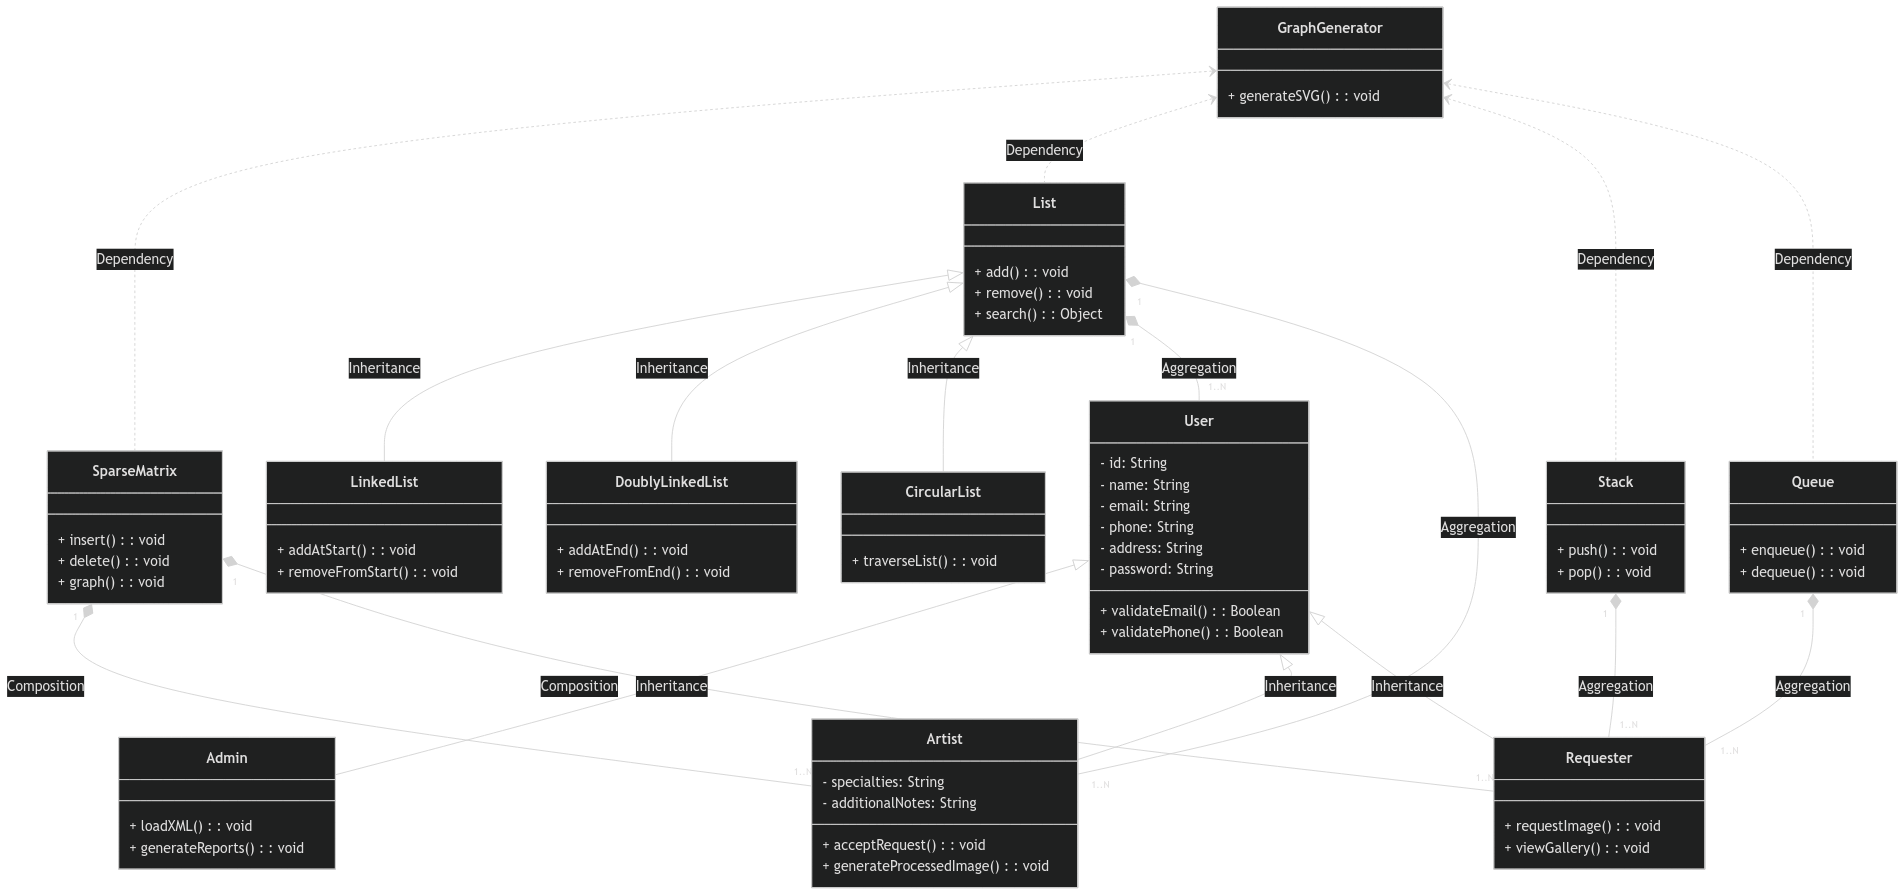
\includegraphics[width=0.2\columnwidth]{images/diagram.png}
        \caption{Captura de pantalla del sistema en ejecución.}
        \label{fig:diagram}
    \end{figure}


    \section*{Referencias}
    \begin{itemize}
        \item Grady Booch, (1994). \textit{Object-Oriented Analysis and Design with Applications}. Benjamin/Cummings Publishing Company.
        \item Robert C. Martin, (2002). \textit{Agile Software Development, Principles, Patterns, and Practices}. Prentice Hall.
        \item E. Gamma, R. Helm, R. Johnson, J. Vlissides. \textit{Design Patterns: Elements of Reusable Object-Oriented Software}. Addison-Wesley.
    \end{itemize}

\end{multicols}

\end{document}